\chapter{Introduction}

\label{chap:intro} 
\epigraph{We choose to go to the moon. We choose to go to the moon in this decade and do the other things, not because they are easy, but because they are hard, because that goal will serve to organize and measure the best of our energies and skills, because that challenge is one that we are willing to accept, one we are unwilling to postpone, and one which we intend to win, and the others, too.}{\textit{John F. Kennedy Moon Speech, Rice Stadium (1962)}}




\section{High Dimensional Non-linear Dynamical Systems}

%Human dreams for the sky, and thus, a better transport vehicle design in a more challenging environments and demanding tasks have never been stopped. 
The need for faster, more efficient and versatile air transport vehicles continues to drive challenging design problems in Aerospace engineering. As examples, the desire to reduce travel time from New York City to London by half has led to silent supersonic commercial aircraft initiated by \textit{Aerion Supersonic}, while \textit{SpaceX} is developing vehicles for space exploration as shown in \cref{fig:intro-backgrounds}.

% show the backgrounds
\begin{figure}[htb]
\centering
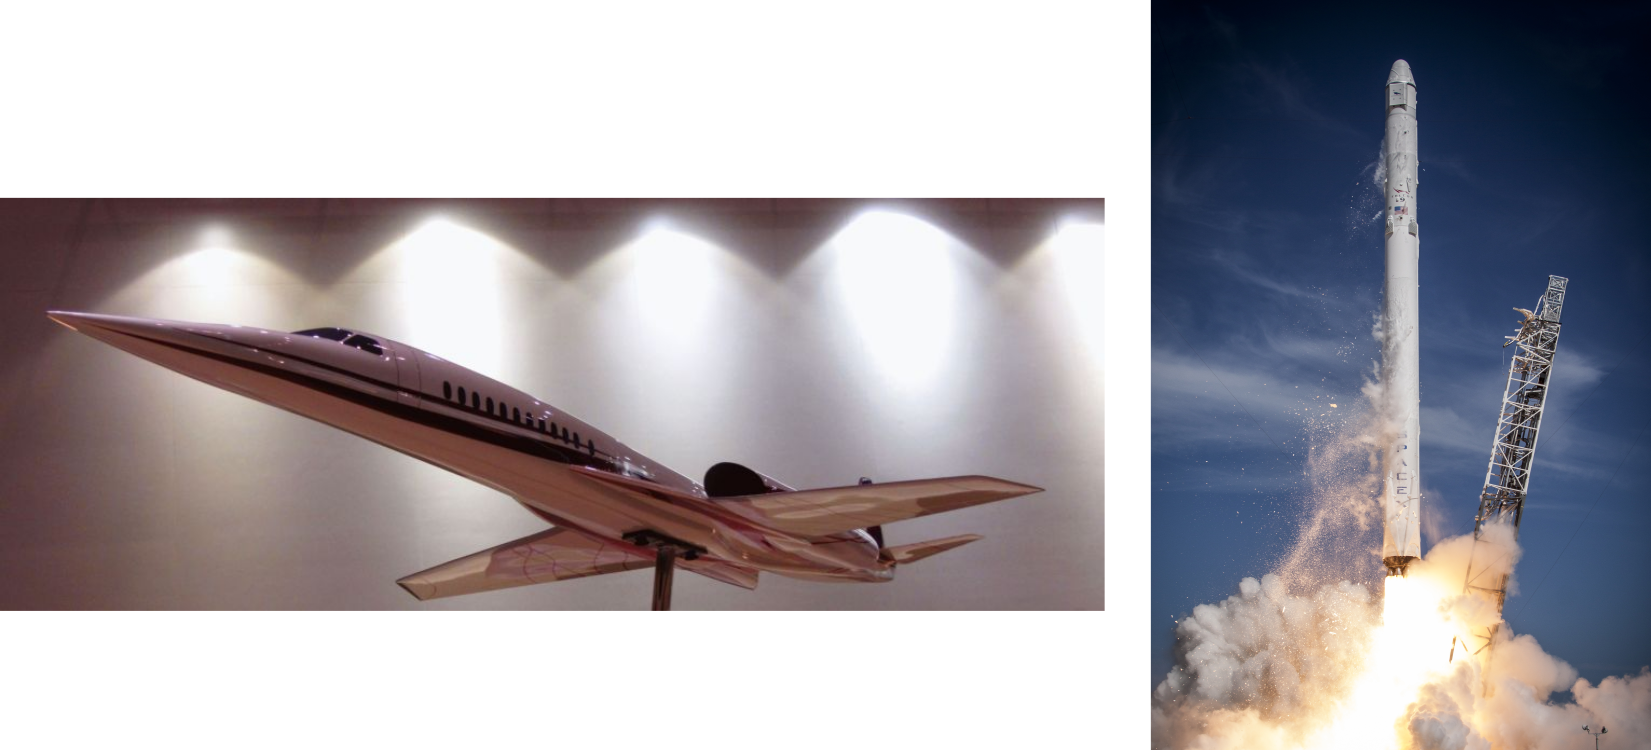
\includegraphics[width=\textwidth]{Intro/intro.png}
\caption{Left: Aerion SBJ designed by jet builder Aerion Supersonic that expects to fly silent supersonic planes by 2024, unlocking a \$40 billion market~\citep{wiki:as2}. Right: Human launch of SpaceX's Falcon 9 rocket raises the company value to \$44 billion~\citep{wiki:fal9}.}
\label{fig:intro-backgrounds}
\end{figure}
